% !TEX root = ../../../main.tex

\toggletrue{image}
\toggletrue{imagehover}
\chapterimage{python_environment}
\chapterimagetitle{\uppercase{Python Environment}}
\chapterimageurl{https://xkcd.com/1987/}
\chapterimagehover{The Python environmental protection agency wants to seal it in a cement chamber, with pictorial messages to future civilizations warning them about the danger of using sudo to install random Python packages.}

\chapter{Parameter}
\label{chapter-parameter}

Wir kennen bereits Funktionen, die beim Funktionsaufruf ein Argument benötigen. Seit dem ersten Kapitel benutzen wir zum Beispiel \lstinline{forward(100)}. Die Zahl \lstinline{100} ist dabei das Argument. Damit man beim Funktionsaufruf ein \textbf{Argument} übergeben kann, muss man bei der Funktionsdefinition einen \textbf{Parameter} definieren. In diesem Kapitel geht es darum, wie man für eigene Funktionen einen Parameter definieren kann. Die Lernziele lauten:

\newcommand{\parameterLernziele}{
\begin{todolist}
\item Sie erklären an einem Beispiel das Prinzip von Parametern.
\item Sie erstellen eine eigene Funktion, welche einen oder mehrere Parameter verwendet.
\item Sie rufen eine eigene Funktion mit einem oder mehreren Parametern auf.
\end{todolist}
}

\lernziel{\autoref{chapter-parameter}, \nameref{chapter-parameter}}{\protect\parameterLernziele}

\parameterLernziele

\section{Drei Quadrate \Ninja[][white]}

Wir können mit dem Programm aus \autoref{lst-drei-quadrate-1} die Figur aus \autoref{figure-drei-quadrate-1} zeichnen.

\begin{figure}[htb]
\centering
\begin{minipage}[c][4cm]{0.4\linewidth}
\centering
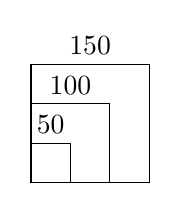
\begin{tikzpicture}
	\draw (0,0) -- ++(0.5cm, 0) -- ++(0, 0.5cm) to node [sloped, above] {$50$} ++(-0.5cm, 0) -- ++(0, -0.5cm);
	\draw (0,0) -- ++(1cm, 0) -- ++(0, 1cm) to node [sloped, above] {$100$}  ++(-1cm, 0) -- ++(0, -1cm);
	\draw (0,0) -- ++(1.5cm, 0) -- ++(0, 1.5cm) to node [sloped, above] {$150$} ++(-1.5cm, 0) -- ++(0, -1.5cm);
\end{tikzpicture}
\caption{Drei \textbf{unterschiedlich} grosse, verschachtelte Quadrate.}
\label{figure-drei-quadrate-1}
\end{minipage}
\hfill
\begin{minipage}[c]{0.55\linewidth}
\centering
\begin{lstlisting}[language=python, caption={Drei Funktionsaufrufe mit Argument (\graybgtexttt{drei\_quadrate\_1.py}).}, label={lst-drei-quadrate-1}]
import turtle as t


def quadrat(seitenlaenge):
    for i in range(4):
        t.fd(seitenlaenge)
        t.lt(90)


quadrat(50)
quadrat(100)
quadrat(150)

t.done()
\end{lstlisting}
\end{minipage}
\end{figure}

Wir können die Seitenlänge der Quadrate auf einfache Weise anpassen, in dem wir bei der Funktionsdefinition einen Parameter notieren (Zeile 4). Dies ist eine spezielle Variable. Beim Funktionsaufruf können wir dann ein Argument (Zeile 10, Zeile 11 und Zeile 12) übergeben.

\section{Parameter definieren}

Wir können in der Funktionsdefinition \textbf{zwischen} den Klammern Parameter definieren.

\begin{definition}[Parameter]
Ein Parameter ist eine spezielle \textbf{Variable} der Funktion. Die Variable ist nur innerhalb der Funktionsdefinition verfügbar. Deshalb ist ein Parameter eine \textbf{lokale Variable}. Man definiert einen Parameter bei der Funktionsdefinition \textbf{zwischen} den runden Klammern. \textbf{Mehrere Parameter} werden durch \textbf{Komma} getrennt.
\end{definition}

\begin{example}
In \autoref{lst-drei-quadrate-1} wird in Zeile vier bei der Funktionsdefinition ein Parameter verwendet. Der Parametername lautet \lstinline{seitenlaenge}.
\end{example}

\begin{important}
Beim Funktionsaufruf muss für \textbf{jeden} Parameter ein \textbf{Argument} vorhanden sein. Man muss jedem Parameter einen Wert übergeben.
\end{important}

\subsection{Wie wählen wir Parameternamen?}

Innerhalb der üblichen Regeln sind wir grundsätzlich frei bei der Wahl des Parameternamens. Jedoch sollte man einen Parameternamen so wählen, dass man allein durch den Parameternamen weiss, wozu der Parameter verwendet wird.

\begin{cleancode}[Sinnvolle Parameternamen]
Wir wählen \textbf{Parameternamen} so, dass wir direkt verstehen, wofür der Parameter eingesetzt werden soll.
\end{cleancode}

\begin{important}
Besitzt eine Funktionsdefinition mehrere Parameter, dann muss jeder Parametername eindeutig sein.
\end{important}

\begin{cleancode}[Snake Case für Parameternamen]
Da ein Parameter eine lokale \textbf{Variable} darstellt, verwenden wir auch für \textbf{Parameternamen} die Snake Case-Notation.
\end{cleancode}

\begin{example}
\lstinline{seitenlaenge} ist ein sinnvoller Name für einen Parameter, da die Funktion ein Quadrat zeichnet. \lstinline{seitenlaengeQuadrat} wäre nicht in Snake Case-Notation und nicht sinnvoll, da die Funktion bereits \lstinline{quadrat} lautet. 
\end{example}

\section{Variablen beim Funktionsaufruf}

Wie bei allen anderen Funktionsaufrufen auch, müssen wir für eigene Funktionen nicht ein \textbf{Literal als Argument} übergeben. Wir können beim Funktionsaufruf auch eine \textbf{Variable} verwenden. Der Inhalt der Variablen wird dabei nicht gelöscht. \autoref{lst-drei-quadrate-2} zeigt, wie wir die Figur aus \autoref{figure-drei-quadrate-1} mit einer \lstinline{for}-Schleife zeichnen können.

\begin{lstlisting}[language=python, caption={Variablen beim Funktionsaufruf in der \lstinline{for}-Schleifen (\graybgtexttt{drei\_quadrate\_2.py}).}, label={lst-drei-quadrate-2}]
import turtle as t


def quadrat(seitenlaenge):
    for i in range(4):
        t.fd(seitenlaenge)
        t.lt(90)


for laenge in [50, 100, 150]:
    quadrat(laenge)

t.done()
\end{lstlisting}

\section{Aufgaben}

In den folgenden Aufgaben setzen Sie sich mit dem Erstellen von eigenen Funktionen mit Parametern auseinander.

\subsection{Aufgabe 1}

Notieren Sie ein Python-Programm, welches mit der Turtle die \textbf{drei gleichseitigen Dreiecke} aus \autoref{figure-drei-dreiecke} zeichnet. Erstellen Sie eine Funktionsdefinition \lstinline{def dreieck(seitenlaenge):} und notieren Sie darin die Funktionsaufrufe zum Zeichnen \textbf{eines gleichseitigen} Dreiecks. Verwenden Sie im \textbf{Funktionskörper} eine \lstinline{for}-Schleife. Rufen Sie die Funktion dann \textbf{dreimal} auf, um die ganze Figur zu zeichnen.

\begin{figure}[htb]
\centering
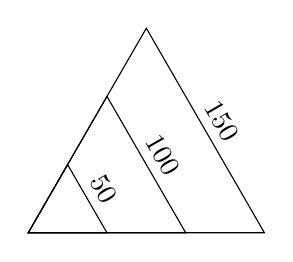
\begin{tikzpicture}
	\draw (0,0) -- ++(1cm, 0) to node [sloped, above] {50} ++(120:1cm) -- cycle;
	\draw (0,0) -- ++(2cm, 0) to node [sloped, above] {100} ++(120:2cm) -- cycle;
	\draw (0,0) -- ++(3cm, 0) to node [sloped, above] {150} ++(120:3cm) -- cycle;
\end{tikzpicture}
\caption{Drei gleichseitige Dreiecke.}
\label{figure-drei-dreiecke}
\end{figure}

\fillwithgrid{\stretch{1}}

\newpage

\subsection{Aufgabe 2}

Notieren Sie ein Python-Programm, welches mit der Turtle die \textbf{vier Kreise} aus \autoref{figure-vier-farbige-kreise} zeichnet. Erstellen Sie eine Funktionsdefinition \lstinline{def kreis(kreisradius):} und notieren Sie darin die Funktionsaufrufe zum Zeichnen \textbf{eines farbigen} Kreises. Die Farbe des Kreises soll \textbf{zufällig} gewählt werden. Rufen Sie die Funktion dann \textbf{viermal} auf, um die ganze Figur zu zeichnen. Verwenden Sie dazu eine \lstinline{for}-Schleife und ein passender \lstinline{range}-Funktionsaufruf.

\begin{figure}[htb]
\centering
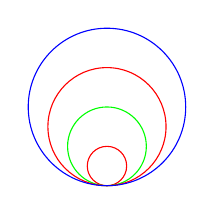
\begin{tikzpicture}
	\draw[red] (0, 0) circle (0.25cm);
	\draw[green] (0, 0.25cm) circle (0.5cm);
	\draw[red] (0, 0.5cm) circle (0.75cm);
	\draw[blue] (0, 0.75cm) circle (1cm);
\end{tikzpicture}
\caption{Vier farbige Kreise.}
\label{figure-vier-farbige-kreise}
\end{figure}

\fillwithgrid{\stretch{1}}

\newpage

\section{Mehrere Parameter}

Wir können beliebig viele Parameter für eine Funktion definieren. Beim Funktionsaufruf spielt die \textbf{Reihenfolge} der Parameter eine Rolle: Die Argumente für die Parameter müssen in derselben Reihenfolge angegeben werden wie die Parameter. \autoref{lst-farbige-quadrate-1} zeigt ein Beispiel mit zwei Parametern. Die Argumente werden beim Funktionsaufruf ebenfalls durch ein Komma getrennt.

\begin{lstlisting}[caption={Funktion mit zwei Parametern (\graybgtexttt{drei\_farbige\_quadrate.py}).}, label={lst-farbige-quadrate-1}]
import turtle as t


def quadrat(seitenlaenge, farbe):
    t.fillcolor(farbe)
    t.begin_fill()
    for i in range(4):
        t.fd(seitenlaenge)
        t.lt(90)
    t.end_fill()
    t.pu()
    t.fd(seitenlaenge + 75)
    t.pd()


quadrat(50, "red")
quadrat(100, "green")
quadrat(150, "blue")

t.done()
\end{lstlisting}

Mit dem Code aus \autoref{lst-farbige-quadrate-1} wird die Figur aus \autoref{figure-drei-farbige-quadrate} erzeugt.

\begin{figure}[htb]
\centering
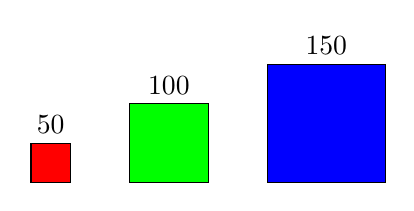
\begin{tikzpicture}
	\draw[fill=red] (0,0) -- ++(0.5cm, 0) -- ++(0, 0.5cm) to node [sloped, above] {$50$} ++(-0.5cm, 0) -- ++(0, -0.5cm);
	\draw[fill=green] (1.25cm,0) -- ++(1cm, 0) -- ++(0, 1cm) to node [sloped, above] {$100$}  ++(-1cm, 0) -- ++(0, -1cm);
	\draw[fill=blue] (3cm,0) -- ++(1.5cm, 0) -- ++(0, 1.5cm) to node [sloped, above] {$150$} ++(-1.5cm, 0) -- ++(0, -1.5cm);
\end{tikzpicture}
\caption{Die Seitenlänge der Quadrate nimmt um 50 zu.}
\label{figure-drei-farbige-quadrate}
\end{figure}

\begin{cleancode}[Leerzeichen 5]
Bei mehreren Parametern folgt \textbf{nach dem Komma} ein Leerzeichen. Beim Funktionsaufruf gilt dies auch für die Argumente.
\end{cleancode}

Wir können natürlich die Funktionsaufrufe auch wieder mit \lstinline{for}-Schleifen lösen, wie in \autoref{lst-farbige-quadrate-2} gezeigt.

\begin{lstlisting}[caption={Eine Schleife mit einer Variablen organisiert die Funktionsaufrufe.}, label={lst-farbige-quadrate-2}]
laenge = 50
for fuellfarbe in ["red", "green", "blue"]:
    quadrat(laenge, fuellfarbe)
    laenge = laenge + 50
\end{lstlisting}

\newpage

\section{Aufgaben}

In den folgenden Aufgaben setzen Sie sich mit dem Erstellen von eigenen Funktionen mit mehreren Parametern auseinander.

\subsection{Aufgabe 1}

Notieren Sie ein Python-Programm, welches ein \textbf{Vieleck} zeichnen kann. Die \textbf{Anzahl der Ecken} und die \textbf{Seitenlänge} sollen flexibel durch jeweils einen Parameter bestimmt werden können. Erstellen Sie eine Funktionsdefinition \lstinline{vieleck} mit zwei Parametern (\lstinline{anzahl} und \lstinline{seite}). Verwenden Sie in der Funktion eine Schleife und rufen Sie die Funktion passend auf, um ein Vieleck mit \textbf{20 Ecken} und einer \textbf{Seitenlänge von 50} zu zeichnen.

\fillwithgrid{3in}

\subsection{Aufgabe 2}

\begin{figure}[htb]
\centering
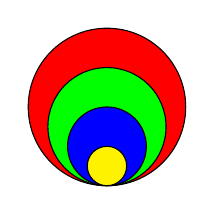
\begin{tikzpicture}
	\draw[fill=red] (0, 0.75cm) circle (1cm);
	\draw[fill=green] (0, 0.5cm) circle (0.75cm);
	\draw[fill=blue] (0, 0.25cm) circle (0.5cm);
	\draw[fill=yellow] (0, 0) circle (0.25cm);
\end{tikzpicture}
\caption{Vier farbig ausgefüllte Kreise.}
\label{figure-vier-farbige-kreise-ausgefuellt}
\end{figure}